\documentclass{standalone}
\usepackage{tikz}
\begin{document}
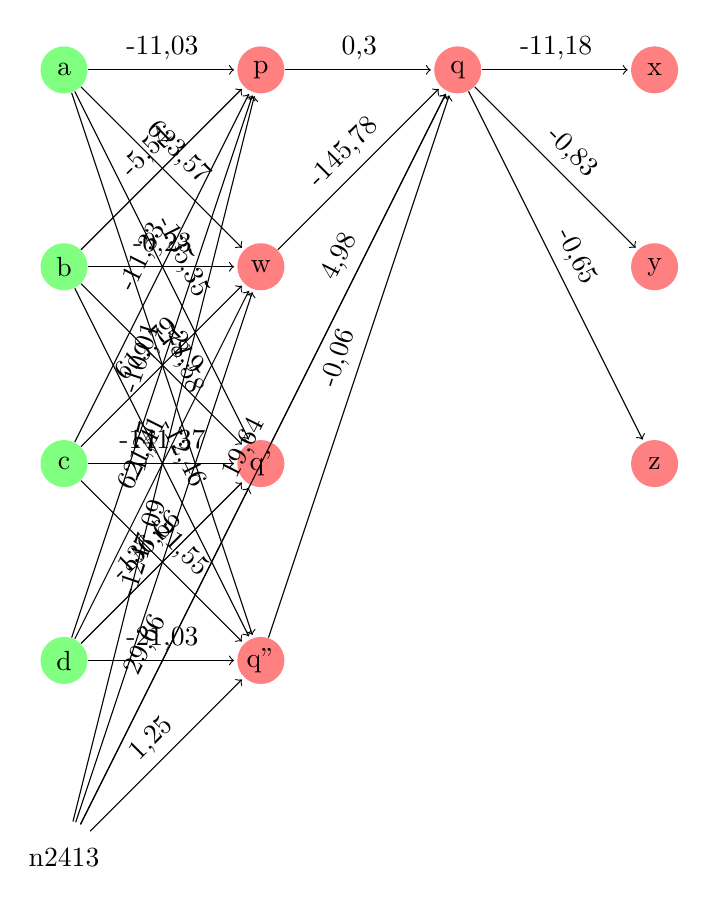
\begin{tikzpicture}[shorten >=1pt,->,draw=black!,node distance=2.5cm]
\tikzstyle{neuron}=[circle,fill=black!25,minimum size=17pt,inner sep=0pt]
\tikzstyle{constant}=[neuron, fill=white!50];
\tikzstyle{sigmoid}=[neuron, fill=red!50];
\tikzstyle{identity}=[neuron, fill=green!50];
\node [identity] (a) {a};
\node [identity,below of=a] (b) {b};
\node [identity,below of=b] (c) {c};
\node [identity,below of=c] (d) {d};
\node [constant,below of=d] (n2413) {n2413};
\node [sigmoid,right of=a] (p) {p};
\node [sigmoid,below of=p] (w) {w};
\node [sigmoid,below of=w] (q') {q'};
\node [sigmoid,below of=q'] (q'') {q''};
\node [sigmoid,right of=p] (q) {q};
\node [sigmoid,right of=q] (x) {x};
\node [sigmoid,below of=x] (y) {y};
\node [sigmoid,below of=y] (z) {z};
\path[every node/.style={sloped,anchor=south,auto=false}]
(q') edge node {4,98} (q)
(w) edge node {-145,78} (q)
(a) edge node {-11,03} (p)
(a) edge node {623,57} (w)
(a) edge node {-135,35} (q')
(a) edge node {-21,58} (q'')
(q) edge node {-11,18} (x)
(q) edge node {-0,83} (y)
(q) edge node {-0,65} (z)
(q'') edge node {-0,06} (q)
(c) edge node {-11,33} (p)
(c) edge node {619,79} (w)
(c) edge node {-141,37} (q')
(c) edge node {-21,55} (q'')
(b) edge node {-5,54} (p)
(b) edge node {-0,23} (w)
(b) edge node {-78,9} (q')
(b) edge node {-12,46} (q'')
(d) edge node {-10,01} (p)
(d) edge node {621,41} (w)
(d) edge node {-136,66} (q')
(d) edge node {-21,03} (q'')
(n2413) edge node {-1247,09} (w)
(n2413) edge node {-1,27} (p)
(n2413) edge node {1,25} (q'')
(n2413) edge node {29,66} (q')
(n2413) edge node {19,64} (q)
(p) edge node {0,3} (q)
;\end{tikzpicture}
\end{document}